El sistema devuelve al usuario datos sobre las acciones que toma cuando estas generan salidas en la consola, se permite realizar una acción, se está realizando una acción o se necesita información que el usuario medio pueda desconocer.

\textbf{Logs de consola: }cuando el sistema realiza un proceso, lo más seguro es que este imprima por pantalla \textit{logs} que puedan resultar informativos.Ver figura.

\begin{figure}[H]
    \begin{center}
    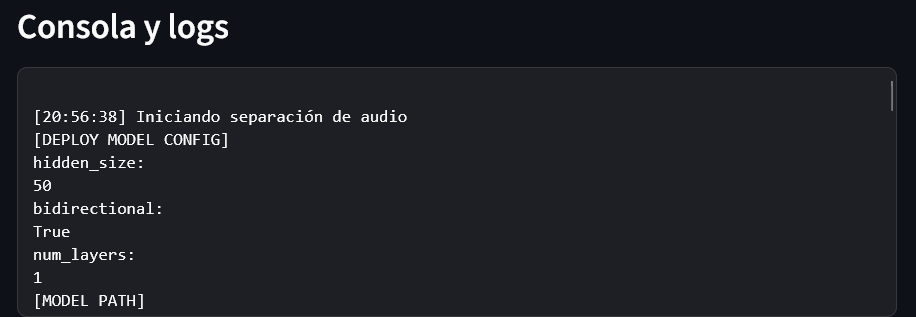
\includegraphics[width=0.7\textwidth]{commons/logs_GUI.png}
    \caption{Ejemplo de \textit{logs} mostrados en la consola de la interfaz}
    \label{fig:logs-gui}
    \end{center}
\end{figure}

\textbf{Mensajes de error: }el usuario puede realizar alguna acción que requiera algún paso previo. Si bien no se ha hecho un estudio exhaustivo de todas las situaciones que puedan desencadenar un error, el sistema muestra mensajes de error en caso de que se produzca un error contemplado. Ver figura.

\begin{figure}[H]
    \begin{center}
    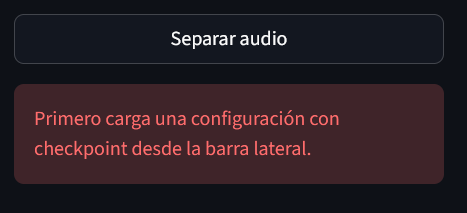
\includegraphics[width=0.7\textwidth]{commons/error_GUI.png}
    \caption{Ejemplo de mensaje de error mostrado en la interfaz al intentar separar una pista sin haber cargado una configuración de modelo previa.}
    \label{fig:error-gui}
    \end{center}
\end{figure}

\textbf{Progreso: }mientras se está realizando una acción que requiere de tiempo, como separar una pista, la interfaz muestra un indicador de espera.Ver figura.

\begin{figure}[H]
    \begin{center}
    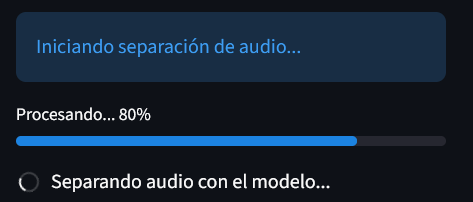
\includegraphics[width=0.7\textwidth]{commons/carga_GUI.png}
    \caption{Ejemplo de indicador de espera en la interfaz mientras se está realizando el proceso de separar una pista.}
    \label{fig:carga-gui}
    \end{center}
\end{figure}

\textbf{Descarga de fuentes: }por cada fuente separada el sistema permite al usuario guardar una copia en su equipo. Esto estaría pensado para una situación real en la que este sistema está \textit{hosteado} en un servidor y no en ejecución local.Ver figura.

\begin{figure}[H]
    \begin{center}
    
\includegraphics[width=0.7\textwidth]{commons/descarga_GUI.png}
    \caption{Botón de la interfaz que descarga un archivo wav de fuente en el almacenamiento del usuario.}
    \label{fig:descarga-gui}
    \end{center}
\end{figure}
